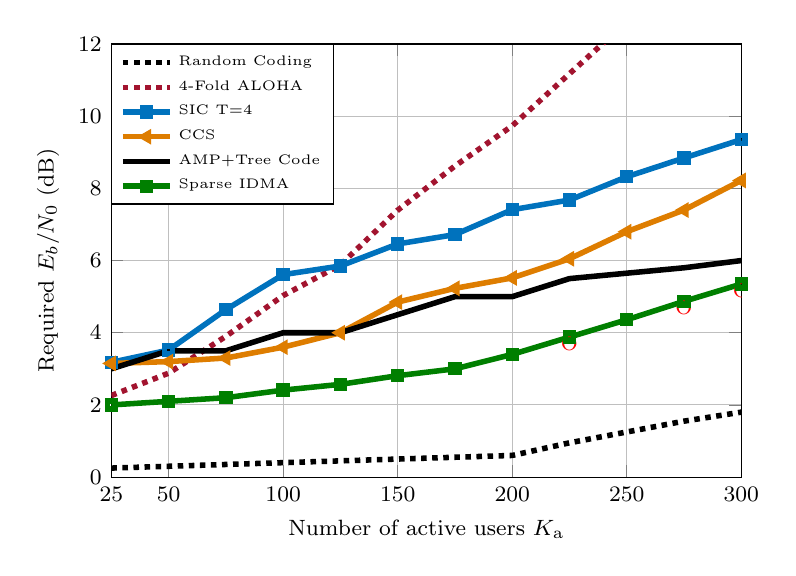
\begin{tikzpicture}
\definecolor{mycolor1}{rgb}{0.63529,0.07843,0.18431}%
\definecolor{mycolor2}{rgb}{0.00000,0.44706,0.74118}%
\definecolor{mycolor3}{rgb}{0.00000,0.49804,0.00000}%
\definecolor{mycolor4}{rgb}{0.87059,0.49020,0.00000}%
\definecolor{mycolor5}{rgb}{0.00000,0.44700,0.74100}%
\definecolor{mycolor6}{rgb}{0.74902,0.00000,0.74902}%

\begin{axis}[%
font=\footnotesize,
width=8cm,
height=5.5cm,
scale only axis,
xmin=25,
xmax=300,
xtick = {25,50,100,...,300},
xlabel={Number of active users $K_{\mathrm{a}}$},
xmajorgrids,
ymin=0,
ymax=12,
ytick = {0,2,...,12},
ylabel={Required $E_b/N_0$ (dB)},
ylabel near ticks,
ymajorgrids,
legend style={font=\tiny, at={(0,1)},anchor=north west, draw=black,fill=white,legend cell align=left}
]

\addplot [color=black,dotted,line width=2.0pt]
  table[row sep=crcr]{
 25	0.25\\
50	0.3\\
75	0.35\\
100	0.4\\
125	0.45\\
150	0.5\\
175	0.55\\
200	0.6\\
225	0.95\\
250	1.25\\
275	1.55\\
300	1.8\\
};
\addlegendentry{Random Coding};

\addplot [color=mycolor1,dotted,line width=2.0pt]
  table[row sep=crcr]{25	2.26\\
50	2.88\\
75	3.9\\
100	5.03\\
125	5.8798\\
150	7.3954\\
175	8.6199\\
200	9.7328\\
225	11.1761\\
250	12.6127\\
275	13.3907\\
300	14.9116\\
};
\addlegendentry{4-Fold ALOHA};

%\addplot [color=mycolor5,dotted,line width=2.0pt]
%  table[row sep=crcr]{25	7.5\\
%35	7.3\\
%50	8.75\\
%100	11.7\\
%150	14.5\\
%200	18\\
%250	21\\
%300	23\\
%};
%\addlegendentry{OP-Exact};

\addplot [color=mycolor2,solid,line width=2.0pt,mark size=1.4pt,mark=square,mark options={solid}]
  table[row sep=crcr]{25	3.18\\
50	3.52\\
75	4.64\\
100	5.61\\
125	5.85\\
150	6.46\\
175	6.72\\
200	7.41\\
225	7.6772\\
250	8.3217\\
275	8.8428\\
300	9.352\\
};
\addlegendentry{SIC T=4};

\addplot [color=mycolor4,solid,line width=2.0pt,mark size=1.3pt,mark=triangle,mark options={solid,rotate=90}]
  table[row sep=crcr]{
  25  3.15\\
50	3.2\\
75	3.3\\
100	3.6\\
125	4\\
150	4.85\\
175	5.23\\
200	5.52\\
225	6.05\\
250	6.8\\
275	7.4\\
300	8.22\\
};
\addlegendentry{CCS};

\addplot [color=black,solid,line width=2.0pt]
  table[row sep=crcr]{
25	3\\
50	3.5\\
75  3.5\\
100	4\\
125	4\\
150 4.5\\
175 5\\
200	5\\
225 5.5
250	5.8\\
275 5.8\\
300	6\\
};
\addlegendentry{AMP+Tree Code};

\addplot [color=mycolor3,solid,line width=2.0pt,mark size=1.4pt,mark=square,mark options={solid}]
  table[row sep=crcr]{
  25  2\\
50	2.1\\
75	2.2\\
100	2.41\\
125	2.57\\
150	2.81\\
175	3\\
200 3.4\\
225 3.88\\
250 4.36\\
275 4.87\\
300 5.35\\
};
\addlegendentry{Sparse IDMA};
\node[] at (axis cs: 300,5.15) {\scriptsize \textcolor{red}{O}};
\node[] at (axis cs: 275,4.69) {\scriptsize \textcolor{red}{O}};
\node[] at (axis cs: 225,3.7) {\scriptsize \textcolor{red}{O}};
%\node[] at (axis cs: 200,4.8) {\scriptsize X};
%\node[] at (axis cs: 200,4.43) {\scriptsize O};
%\addplot [color=black,mark size=2.0pt,only marks,mark=square,mark options={solid}]
%table[row sep=crcr]{
%200 4.43\\
%};
%\node[] at (axis cs: 200,4.43) {\footnotesize O};

%\addplot [color=mycolor6,mark size=6.0pt,only marks,mark=x,mark options={solid},forget plot]
%  table[row sep=crcr]{200	4.8\\
%};
%
%\addplot [color=mycolor5,mark size=5.0pt,only marks,mark=+,mark options={solid},forget plot]
%  table[row sep=crcr]{200	4.43\\
%};

\end{axis}

%\addplot [color=red,solid,line width=2.0pt,mark size=3.5pt,mark=diamond,mark options={solid}]
%  table[row sep=crcr]{25	3.9849\\
%50	5.6396\\
%75	6.2855\\
%100	6.7952\\
%125	7.5262\\
%150	8.3122\\
%175	9.1418\\
%200	10.103\\
%225	11.062\\
%250	12.279\\
%275	13.296\\
%300	14.6648\\
%};
%\addlegendentry{SIC T=2};

%\addplot [color=mycolor3,solid,line width=2.0pt,mark size=2.0pt,mark=+,mark options={solid}]
%  table[row sep=crcr]{25	4.4\\
%50	4.8\\
%75	5.16\\
%100	5.5\\
%125	5.85\\
%150	6.9\\
%175	7.5\\
%200	7.95\\
%225	8.7\\
%250	9.4167\\
%275	10.2773\\
%300	11.37\\
%};
%\addlegendentry{Proposed Scheme, 0 iterations};

\end{tikzpicture}%

